\clearpage
\section{Trigger efficiencies}
\label{app_trigger}

Studies on performance and efficiency have been done for several single-lepton, dilepton and \met\ triggers Results are shown here.

\begin{figure}[h!]
\centering
\subfigure{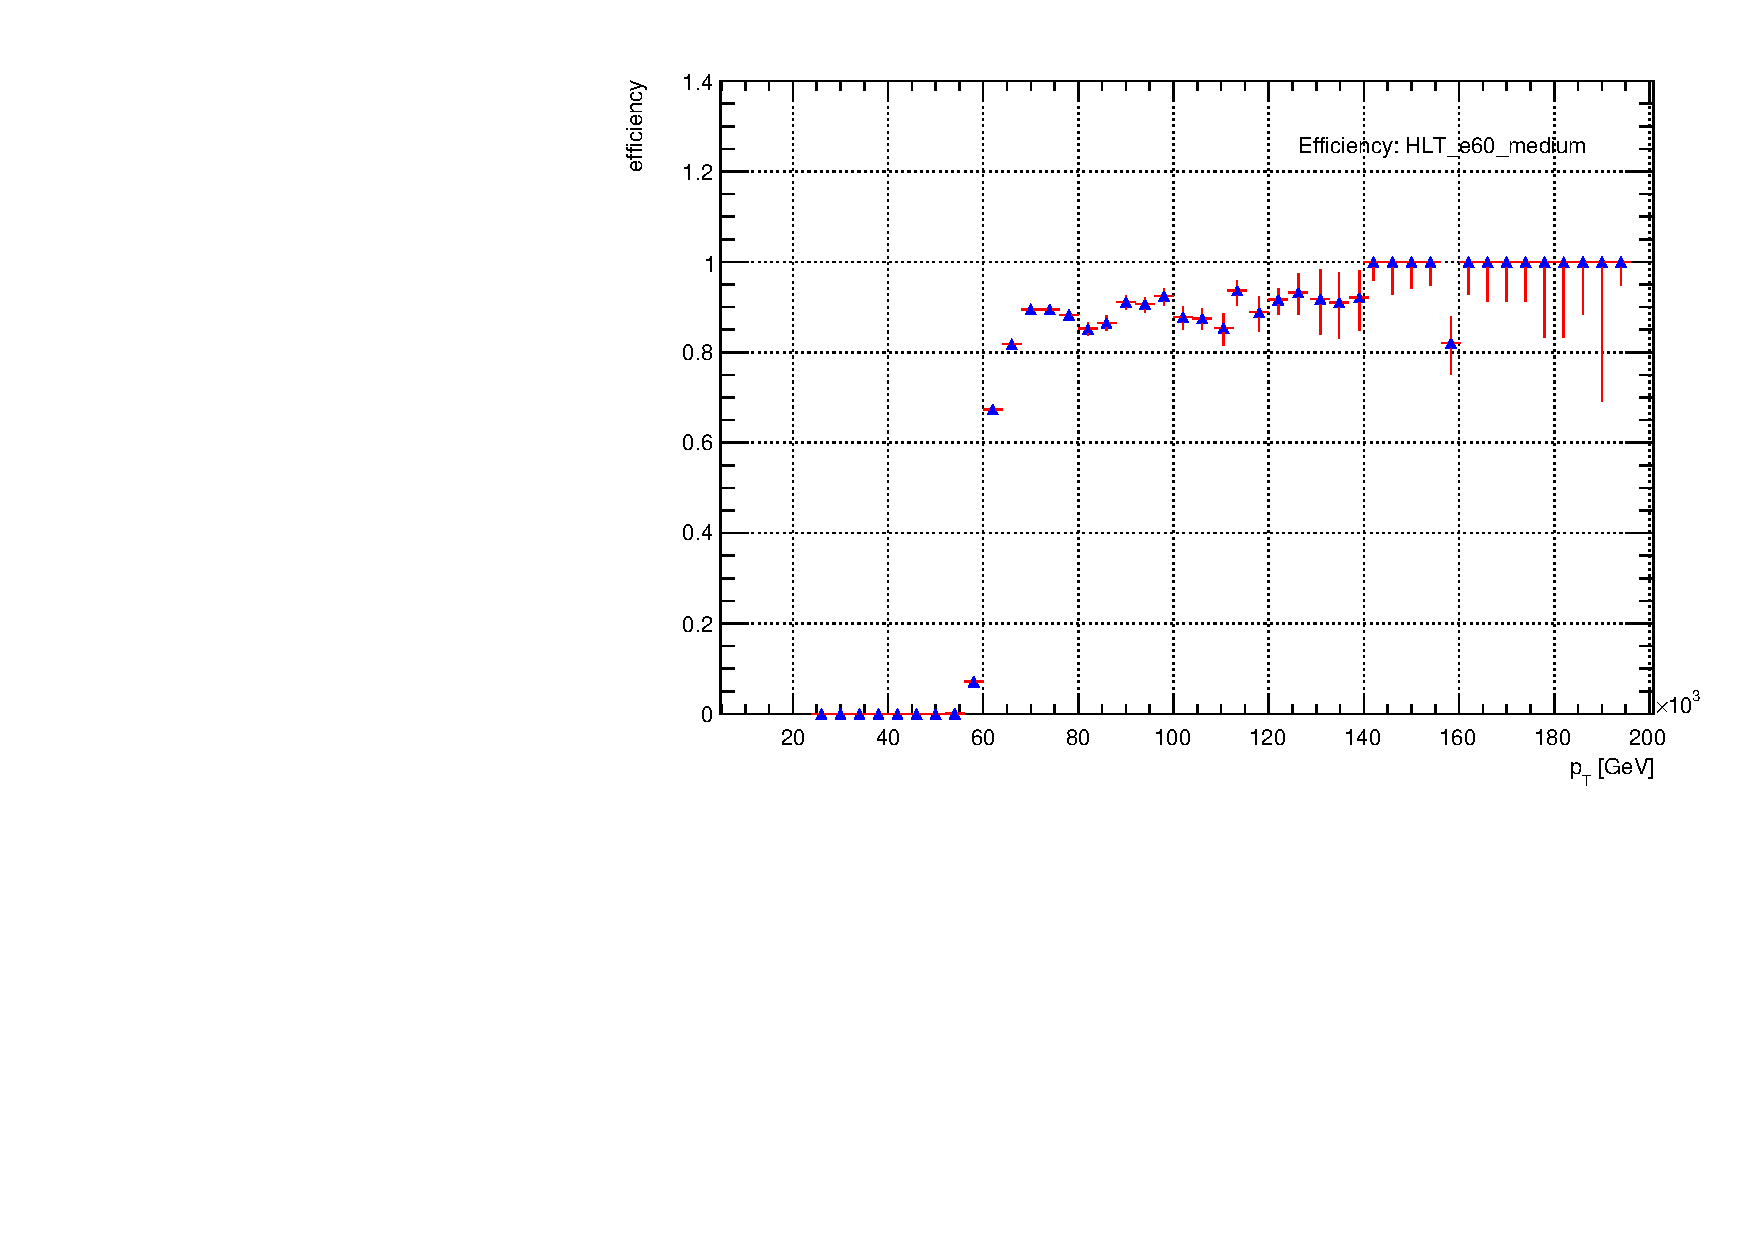
\includegraphics[width=0.45\textwidth]{TRIGGER/Eff_HLT_e60_medium}}
\subfigure{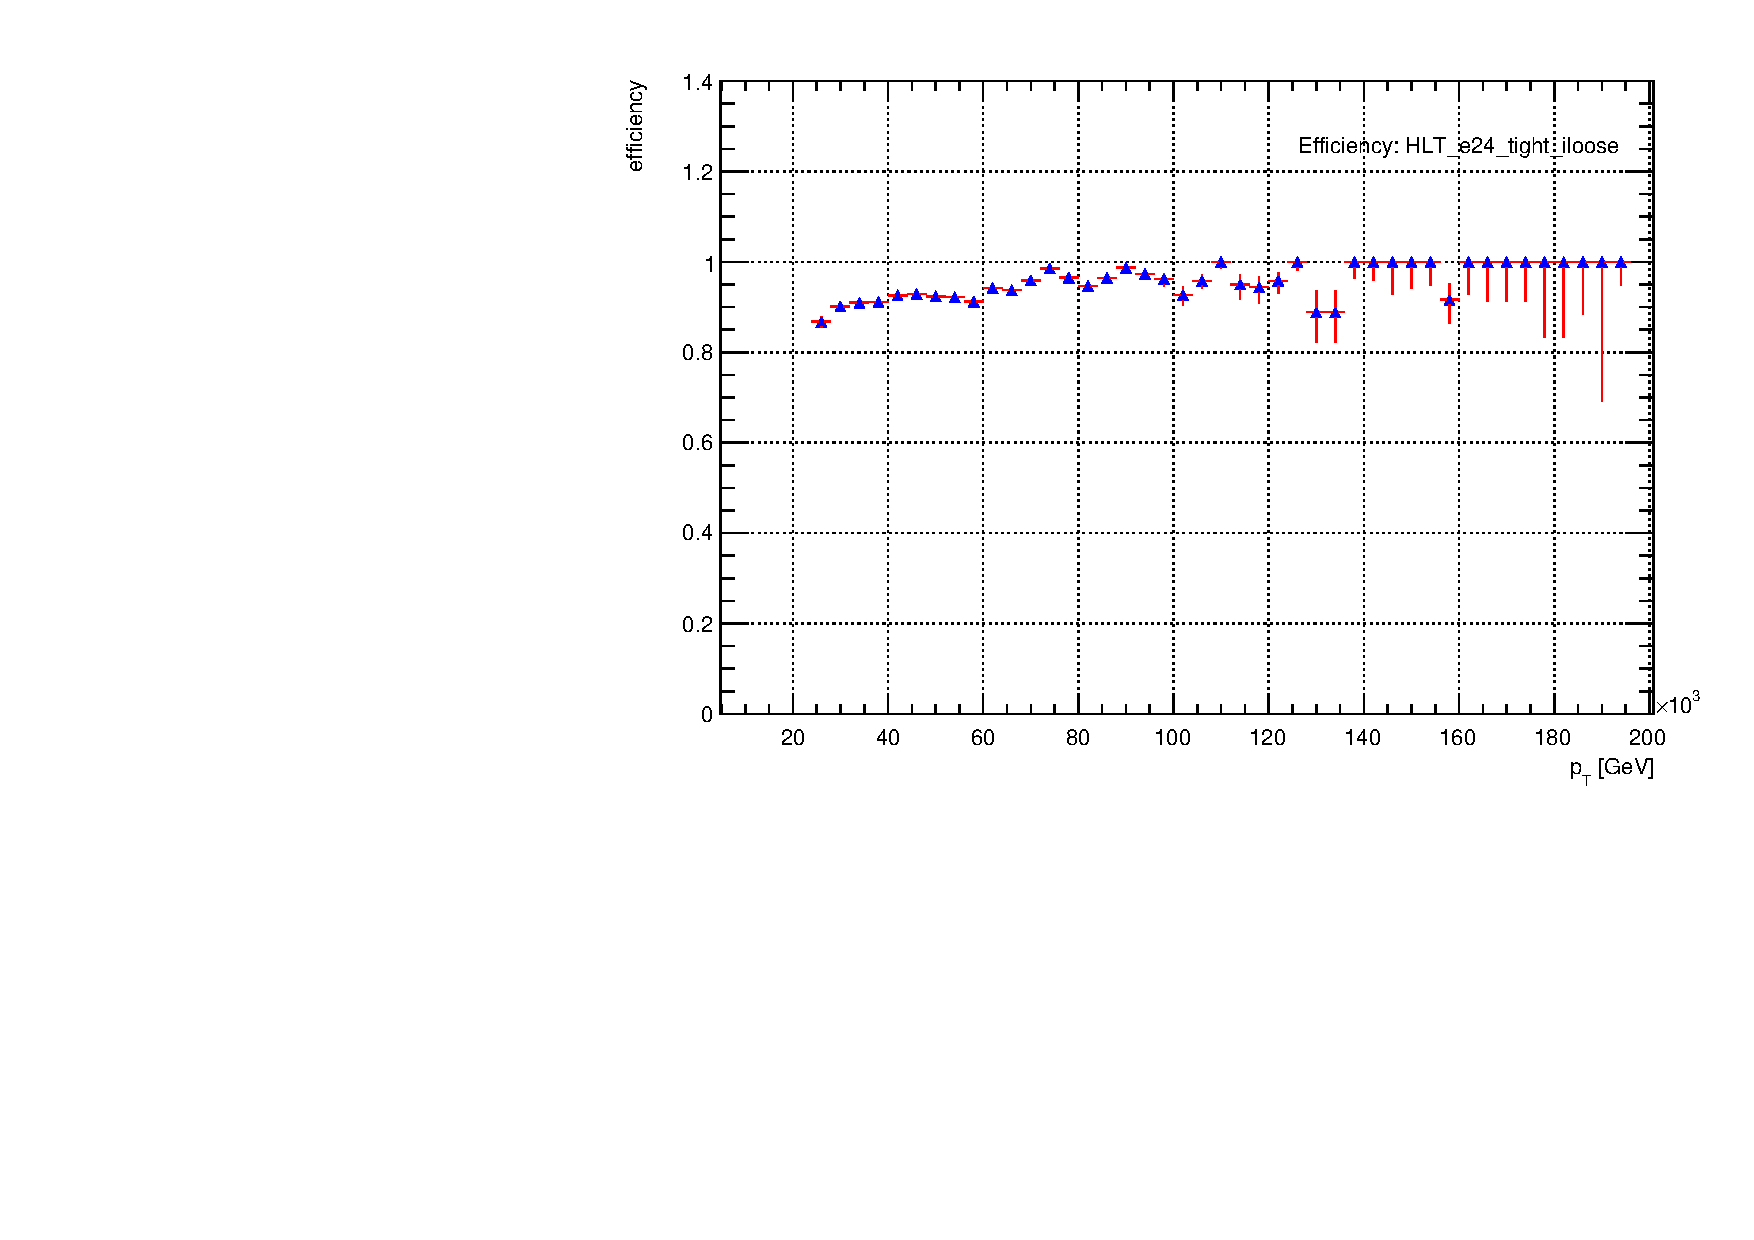
\includegraphics[width=0.45\textwidth]{TRIGGER/Eff_HLT_e24_tight_iloose}}
\caption{Trigger efficiencies for \texttt{HLT\_e60\_medium} and \texttt{HLT\_e24\_tight\_iloose} versus \pt\ of the leading electron.}
\label{fig:eff_trigger_el1}
\end{figure}

\begin{figure}[h!]
\centering
\subfigure{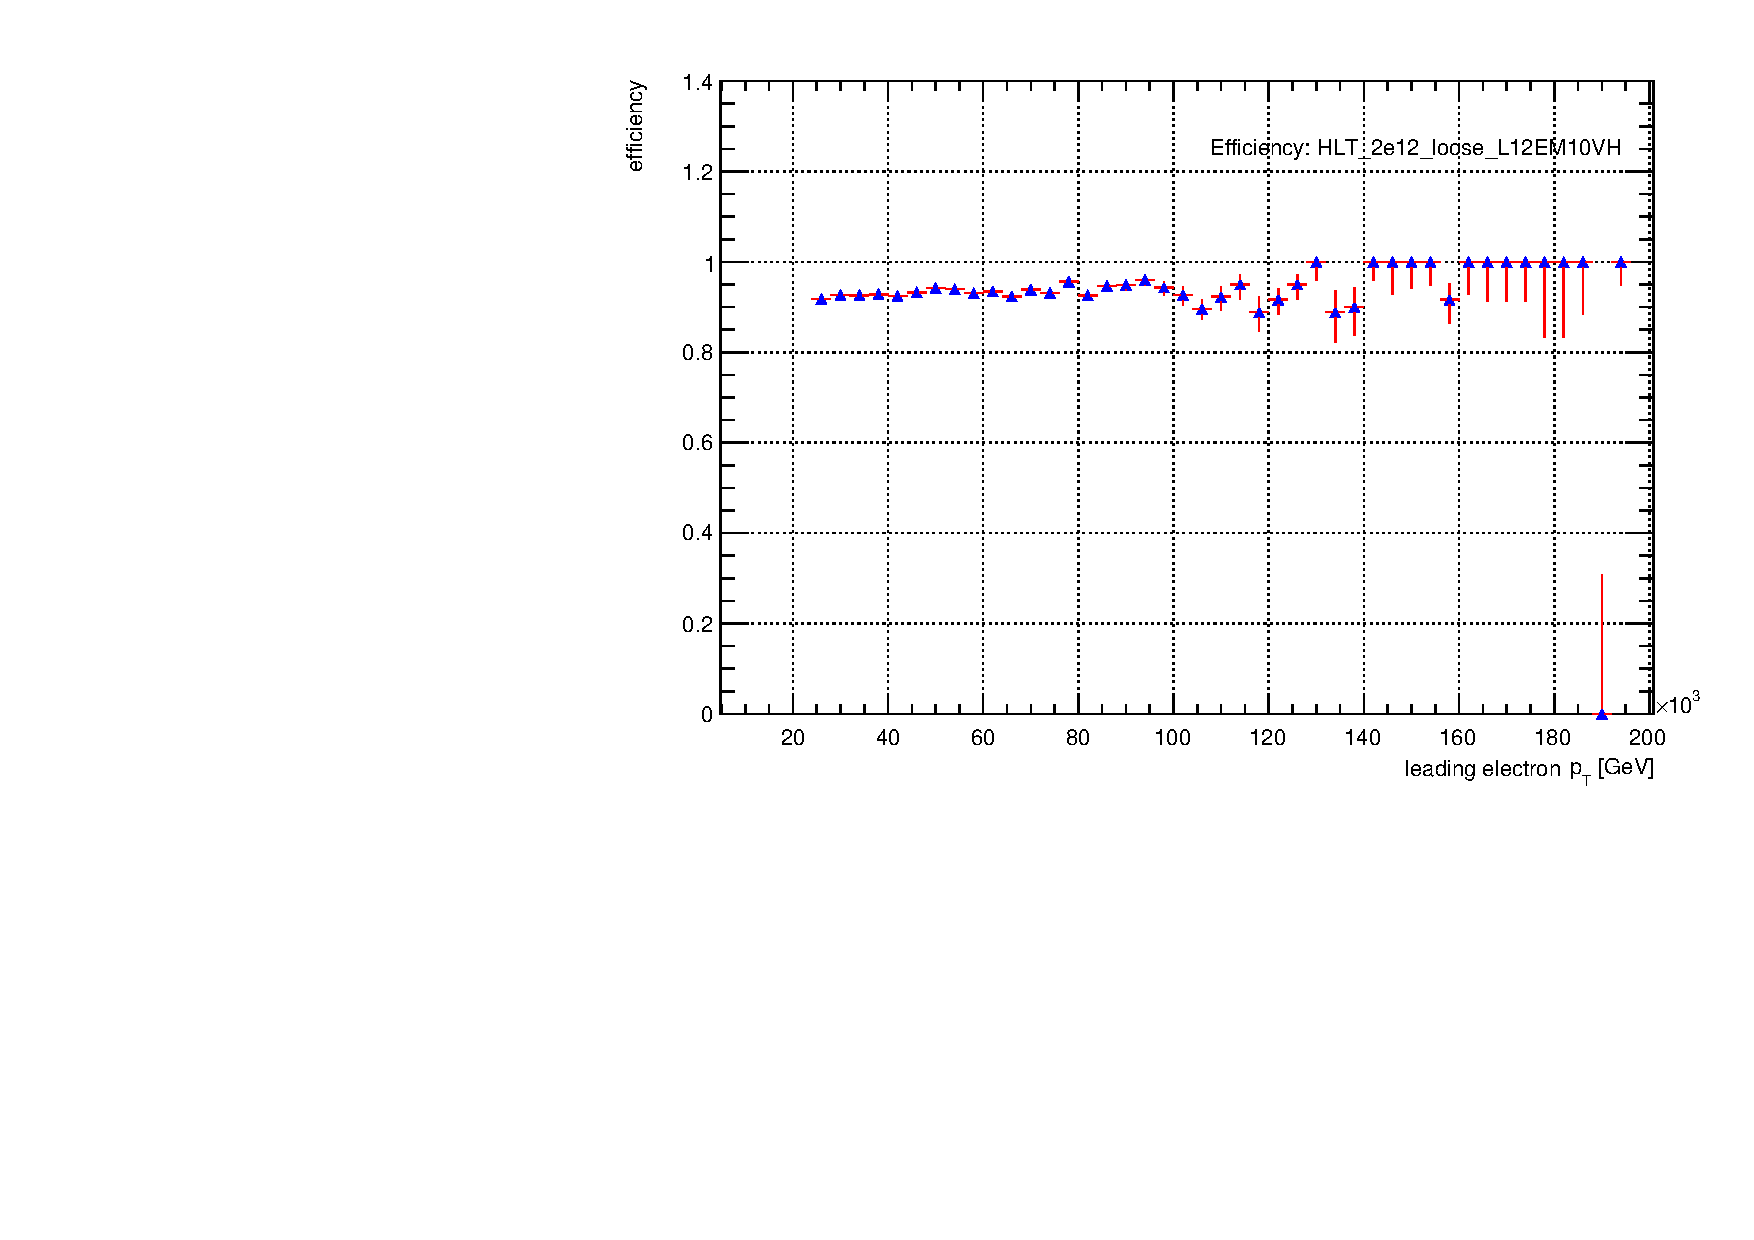
\includegraphics[width=0.45\textwidth]{TRIGGER/Eff_HLT_2e12_loose}}
\subfigure{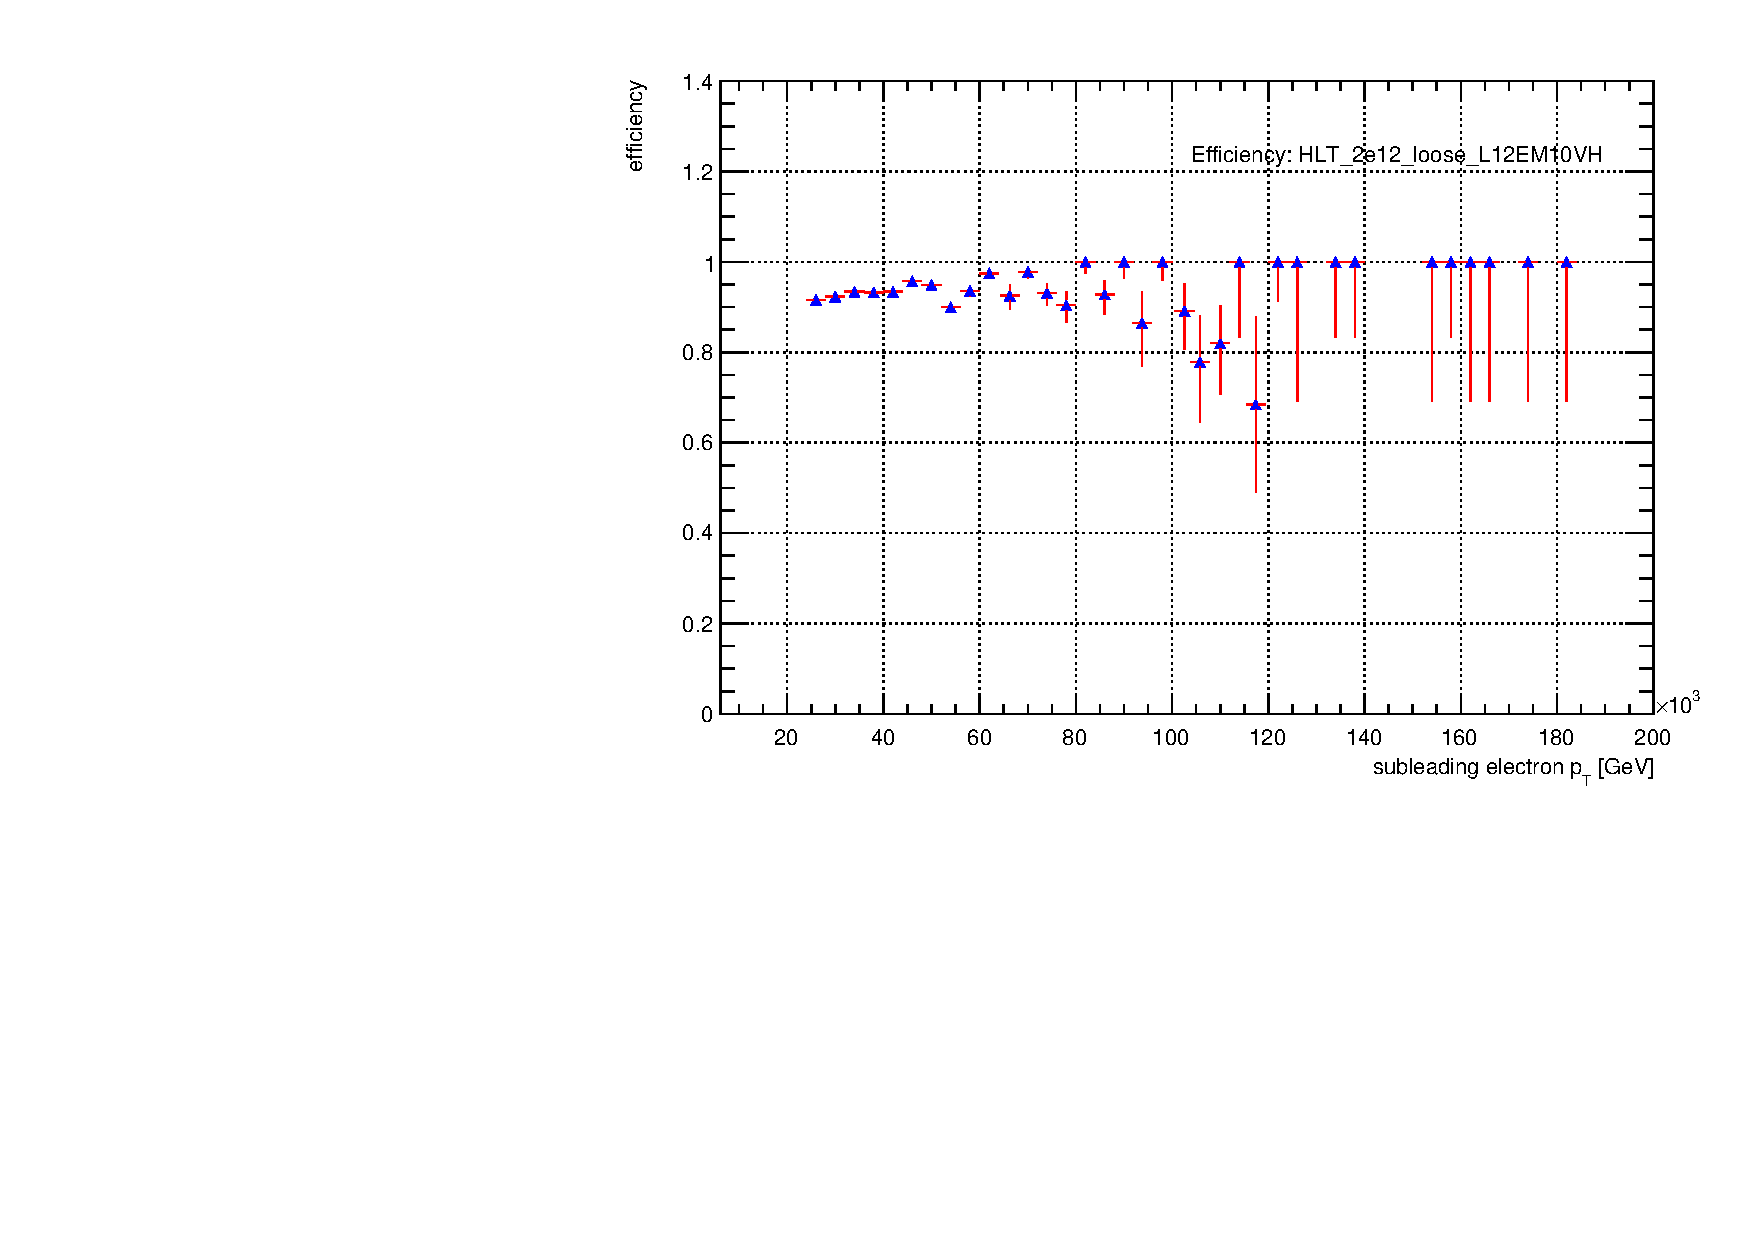
\includegraphics[width=0.45\textwidth]{TRIGGER/Eff_HLT_2e12_loose2}}
\caption{Trigger efficiency for \texttt{HLT\_2e12\_loose\_L12EM10VH} plotted against \pt\ of the leading electron (left-hand side) and the subleading electron (right-hand side).}
\label{fig:eff_trigger_el2}
\end{figure}


\begin{figure}[h!]
\centering
\subfigure{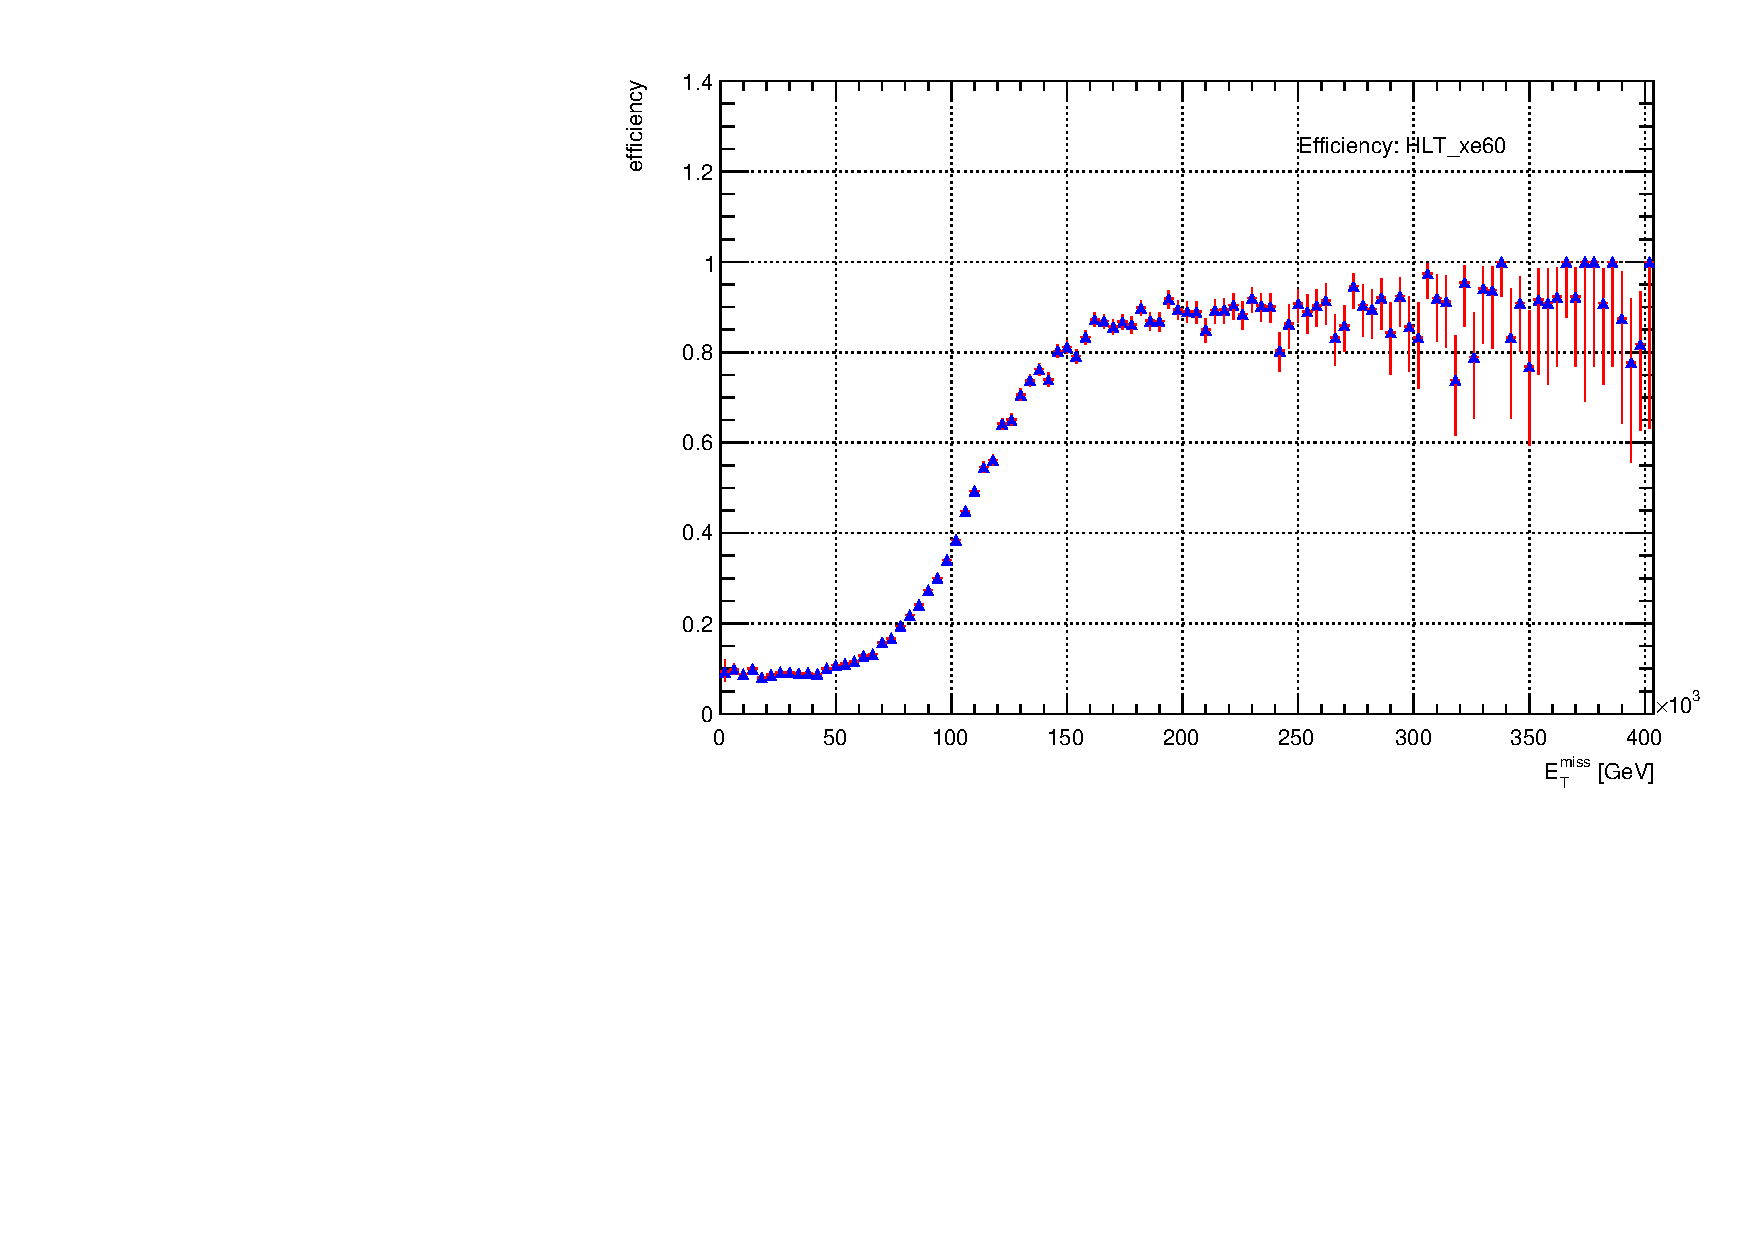
\includegraphics[width=0.45\textwidth]{TRIGGER/Eff_HLT_xe60}}
\subfigure{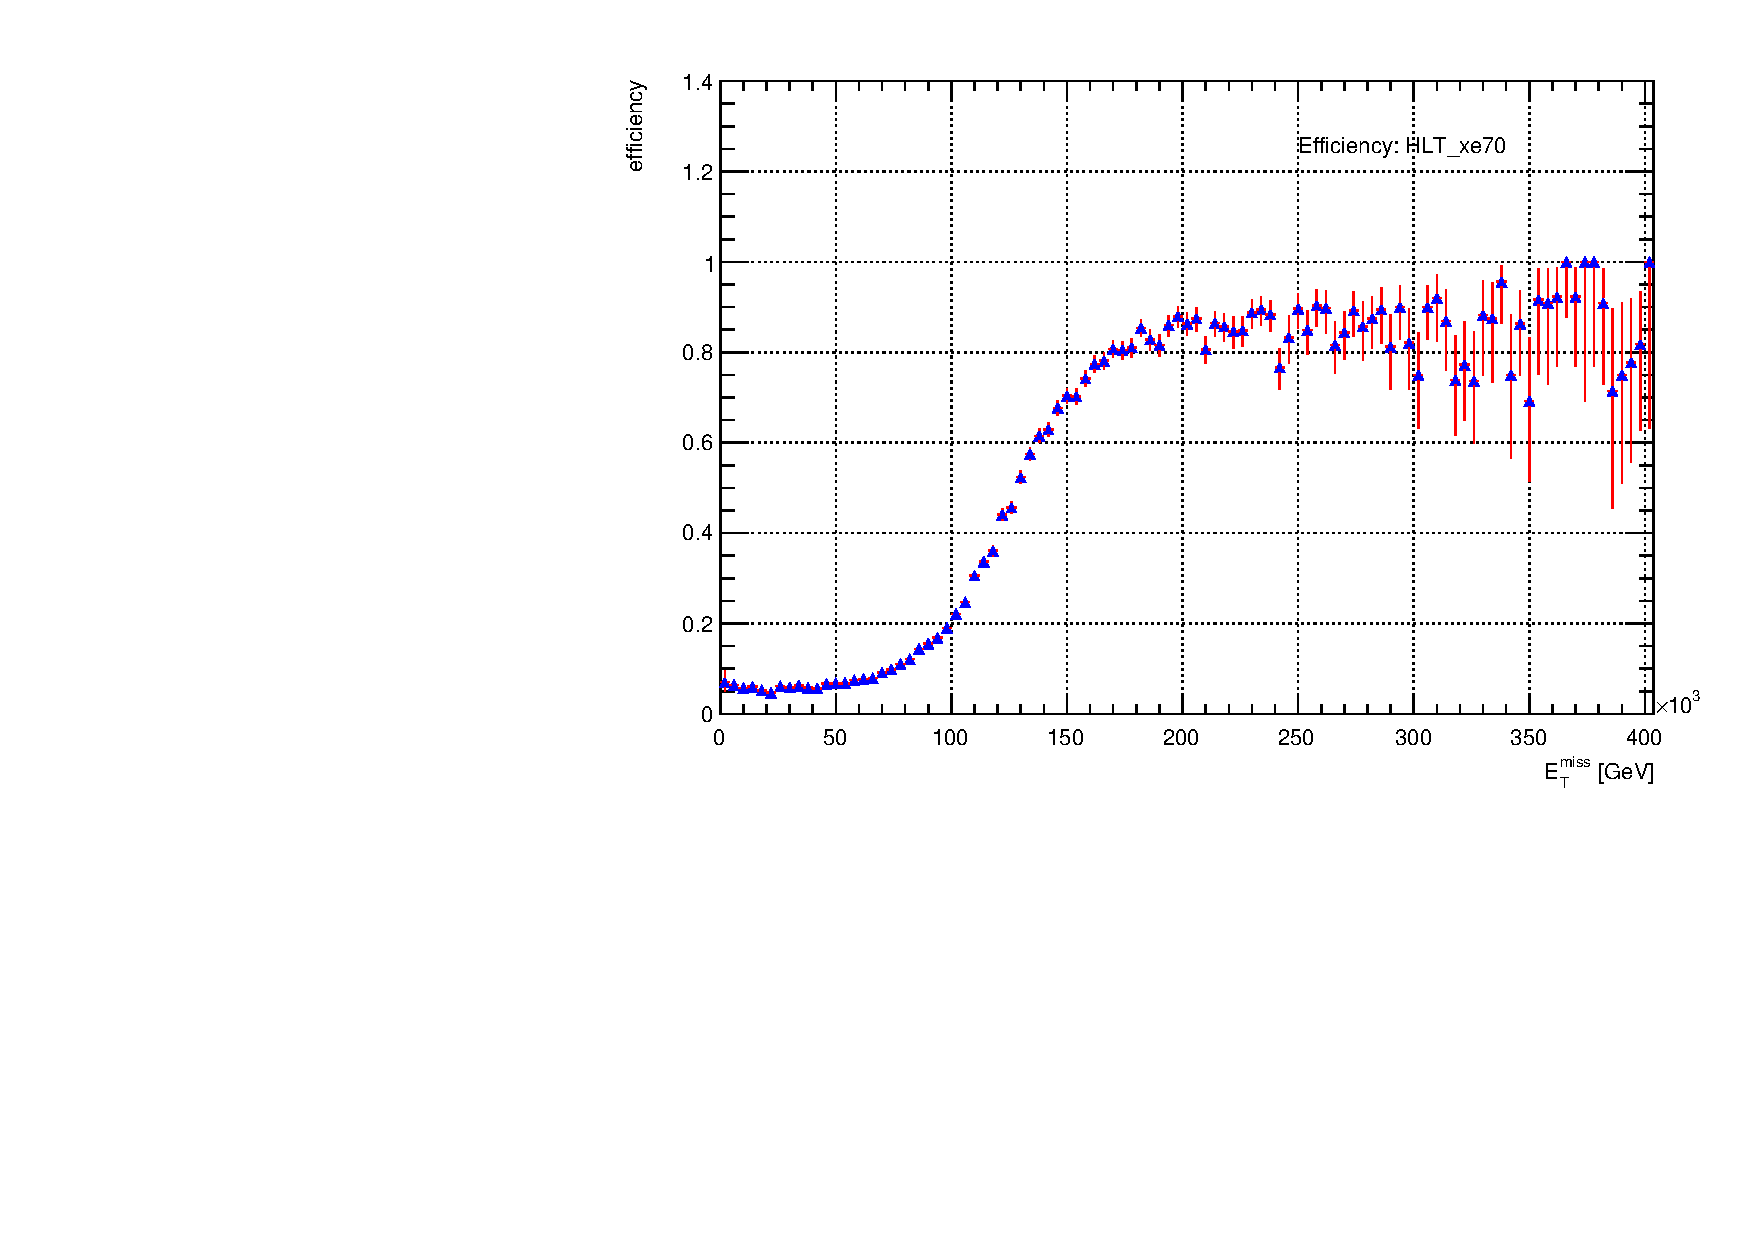
\includegraphics[width=0.45\textwidth]{TRIGGER/Eff_HLT_xe70}}
\caption{Trigger efficiencies for \texttt{HLT\_xe60} and \texttt{HLT\_xe70} versus the missing transverse energy.}
\label{fig:eff_trigger_met}
\end{figure}


\begin{figure}[h!]
\centering
\subfigure{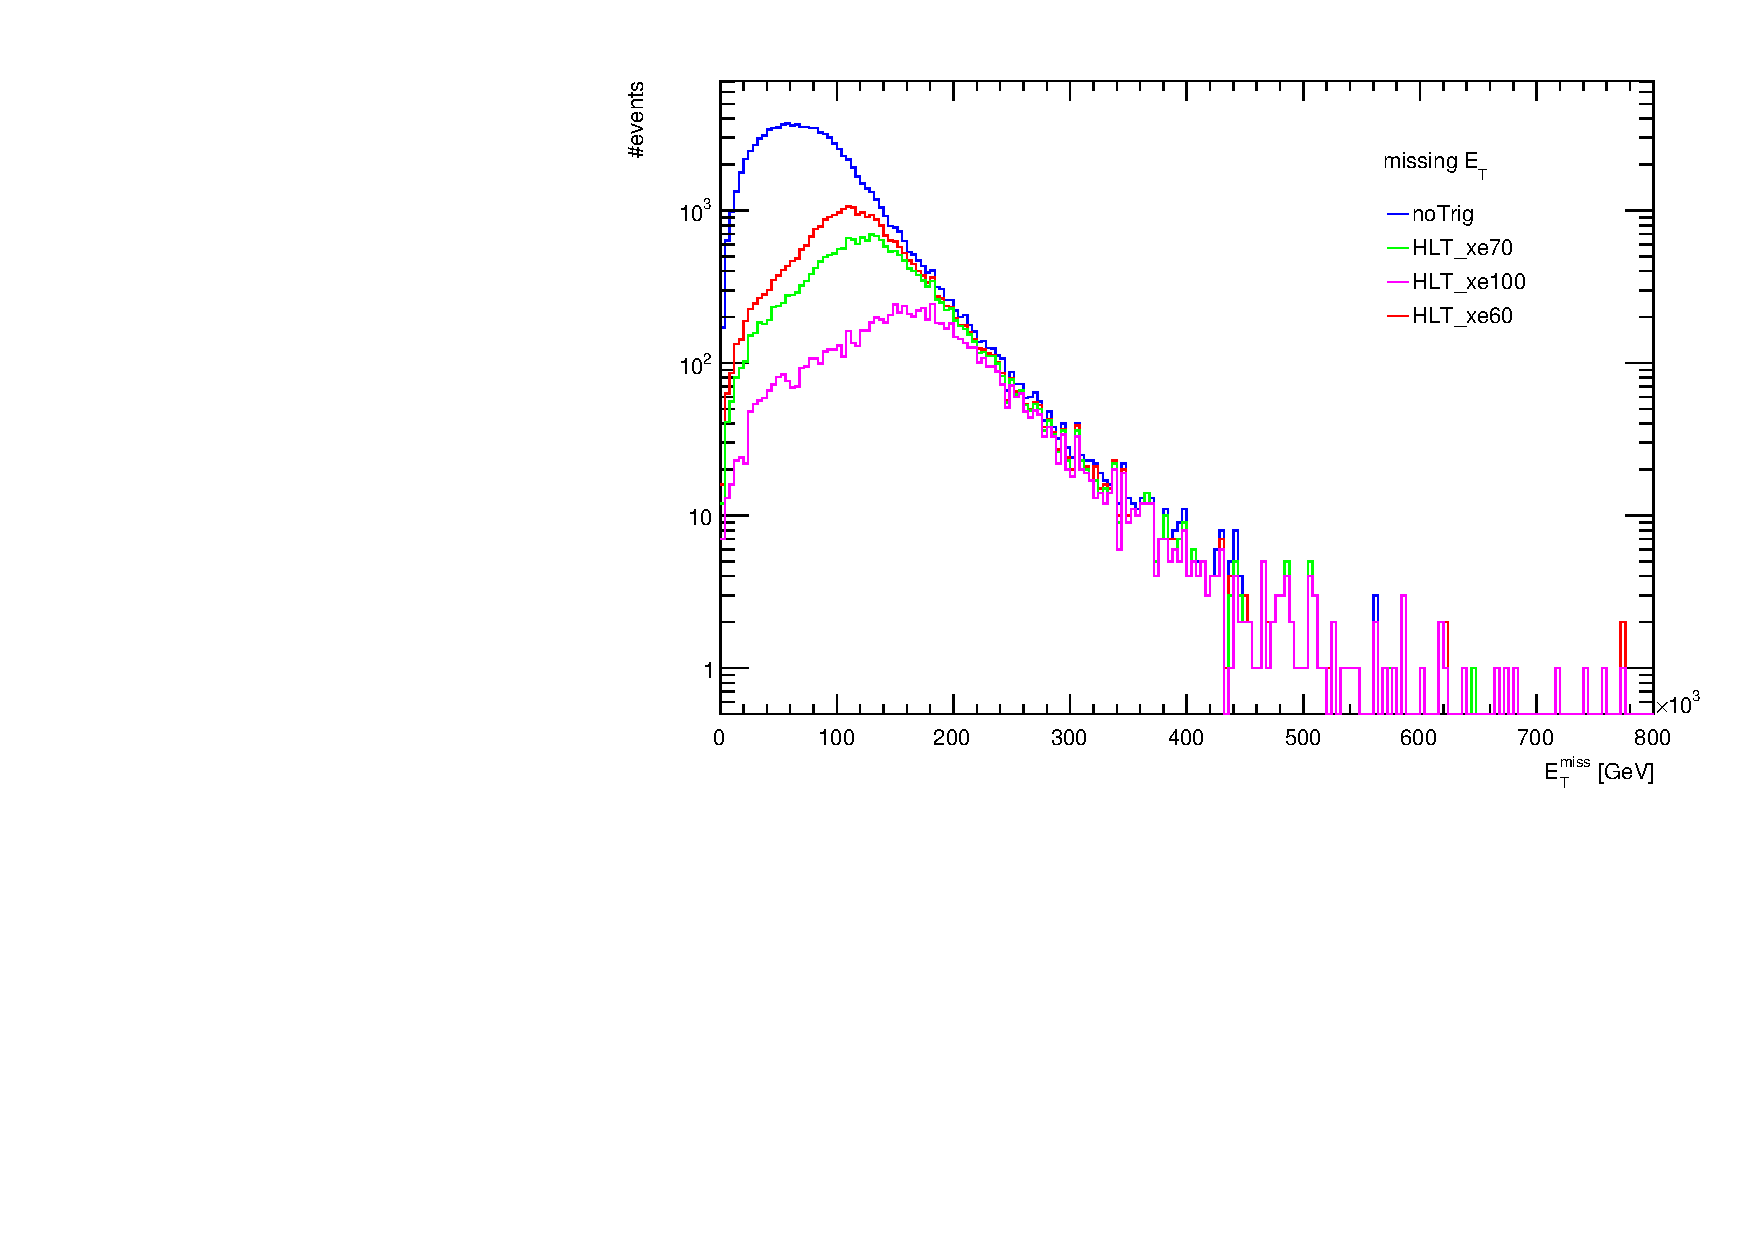
\includegraphics[width=0.6\textwidth]{TRIGGER/Comparison_Met}}
\caption{Events selected by different \met\ triggers and without any trigger selection versus the missing transverse energy.}
\label{fig:dummy_label}
\end{figure}

\begin{figure}[h!]
\centering
\subfigure{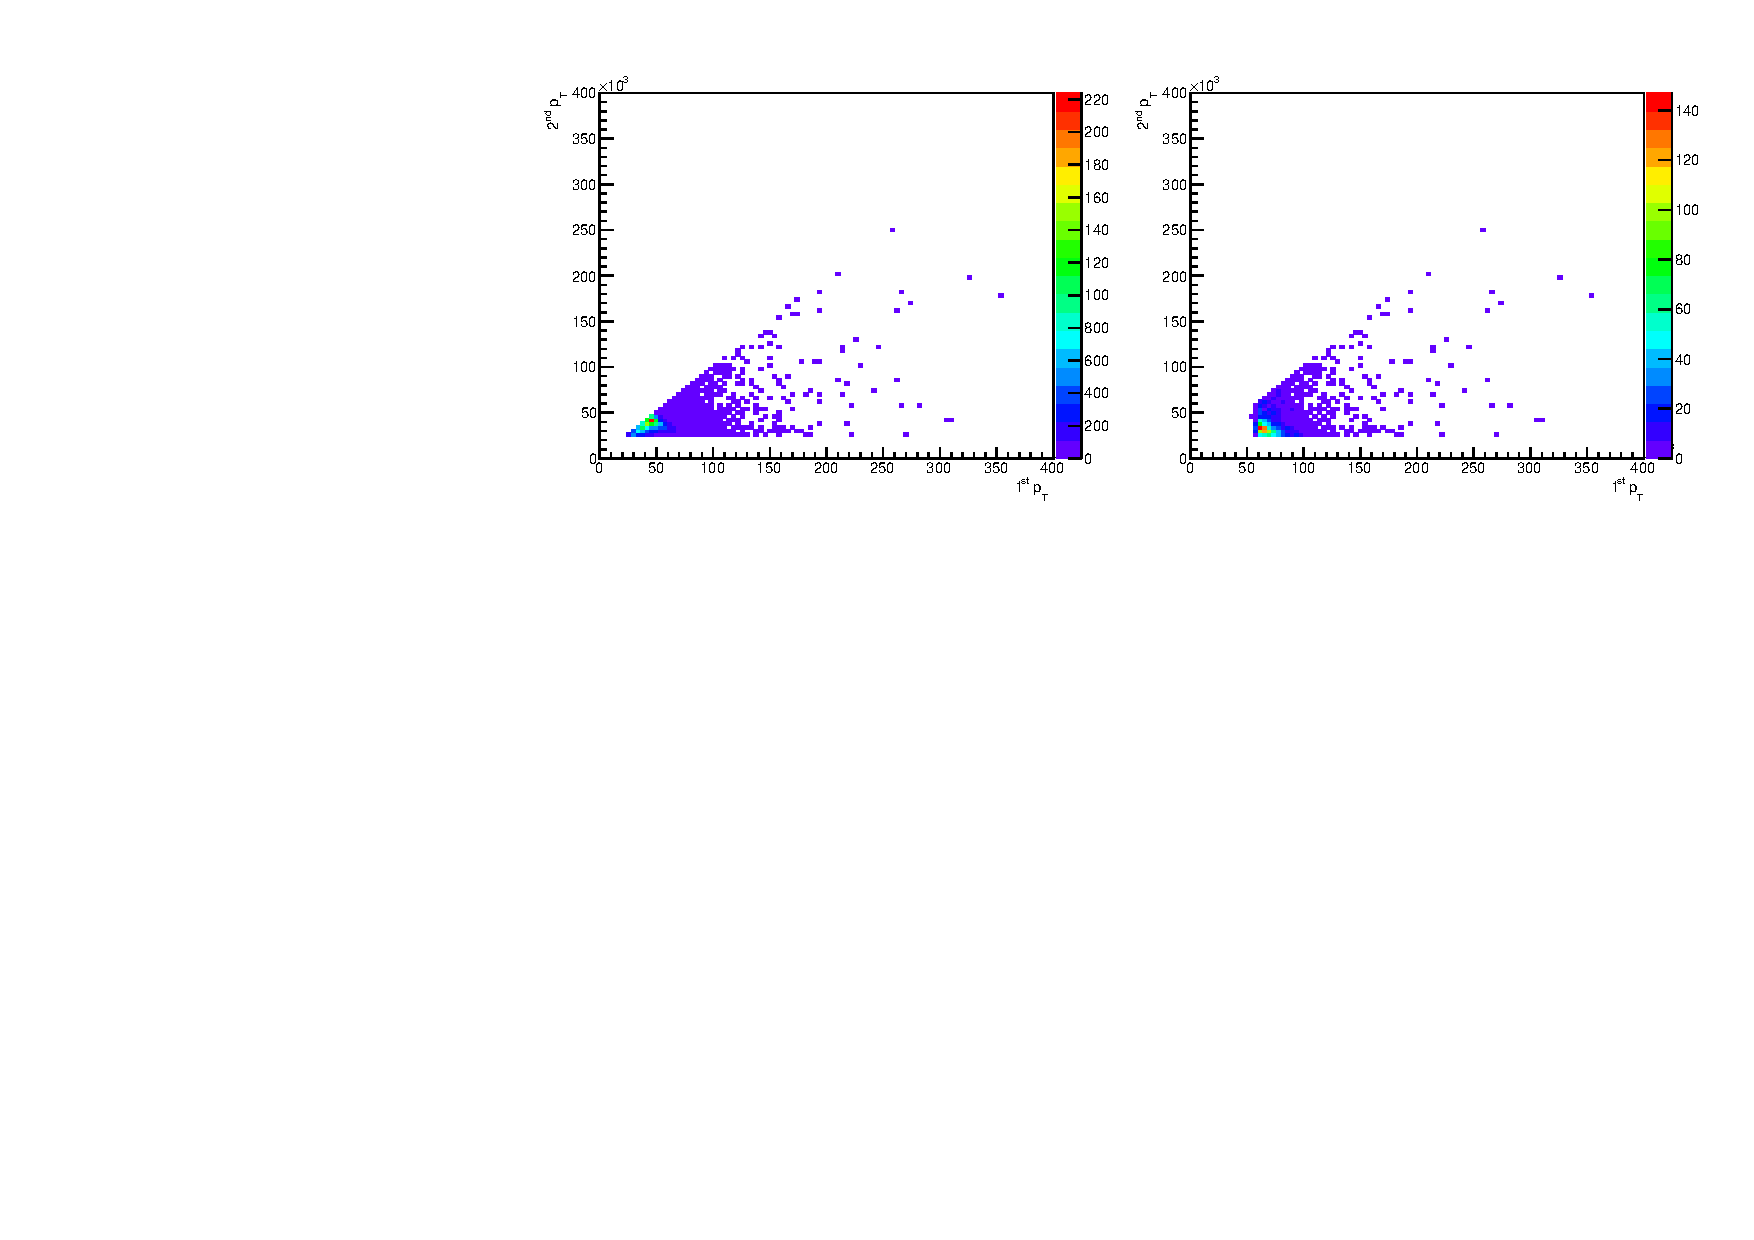
\includegraphics[width=1\textwidth]{TRIGGER/Comparison_e2D}}
\caption{Leading electron versus subleading electron for events selected by \texttt{HLT\_e20\_medium} (left-hand side) and by \texttt{HLT\_e60\_medium} (right-hand side).}
\label{fig:eff_trigger_el2D}
\end{figure}
